\section{Smart meter context model}

\begin{figure}
  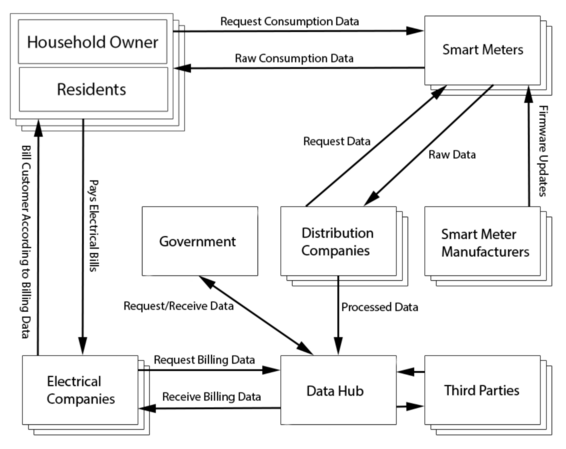
\includegraphics[width=\textwidth]{system}
  \caption{The system}
  \label{contextual:system}
\end{figure}
Legend:

\begin{tabular}{l | l}
  S  & State \\
  L & Power Deliverance company\\
  P & Power production company\\
  D & Power distribution company\\
  DH & Datahub \\
  SM & Smart meter\\
  F & Consumer\\
  SA & Smart appliance\\
  HP & Home production\\
\end{tabular}


\paragraph{} The system is pictured in \cref{contextual:system}.
Inside the house of the consumer the smart meter is placed.

\paragraph{Data connections}
The green lines indicate information flow between actors in the system.
The consumer can interact with the smart meter in order to control smart appliances and monitor the production of his home production devices.

The Datahub stores the comsumption data of the consumer.
This data is available for the consumer, the power distribution company and the power deliverance company.
These three actors have permission to see the consumption data in different granularities.

The consumer can see the data in the finest granularity, whereas the power distribution and the power deliverance company has accesss to a coarser granularity that makes it possible for them to calculate the bill etc.

The distribution company sends price information to the datahub which the consumer then downloads to his smart meter.

\paragraph{Power connections}
The red lines indicate how the power is tranferred from the power production company to the appliances of the consumer.
Unless the consumer has not paid his bills the distribution company distributes power to the house of the consumer.
The smart meter then distributes the power to the installations of the house, including smart appliances controlled by the consumer.
If the consumer has a home production device like a windmill the smart meter will control the usage of the generated power.

\subsection{Actors and threats}
Placing a smart meter in a consumers home and simultaneously requiring external access to its data is a complicated task with many potential risks.
\Cref{contextual:sm_model} represents this context and the actors therein.
This will be used as an offset for a brainstorm that maps the potential attacks on the system.\mikkel{Ref til tables eller lign.}

The actors represented in \cref{contextual:sm_model} are not representative of the complete set of actors having some interaction with the system.
However these other actors communicate with the system through the smart meter and to not clutter the visual representation they have not been included.
They will still be listed as actors below and possible threats to/from them will be considered.

\begin{figure}
  \centering
  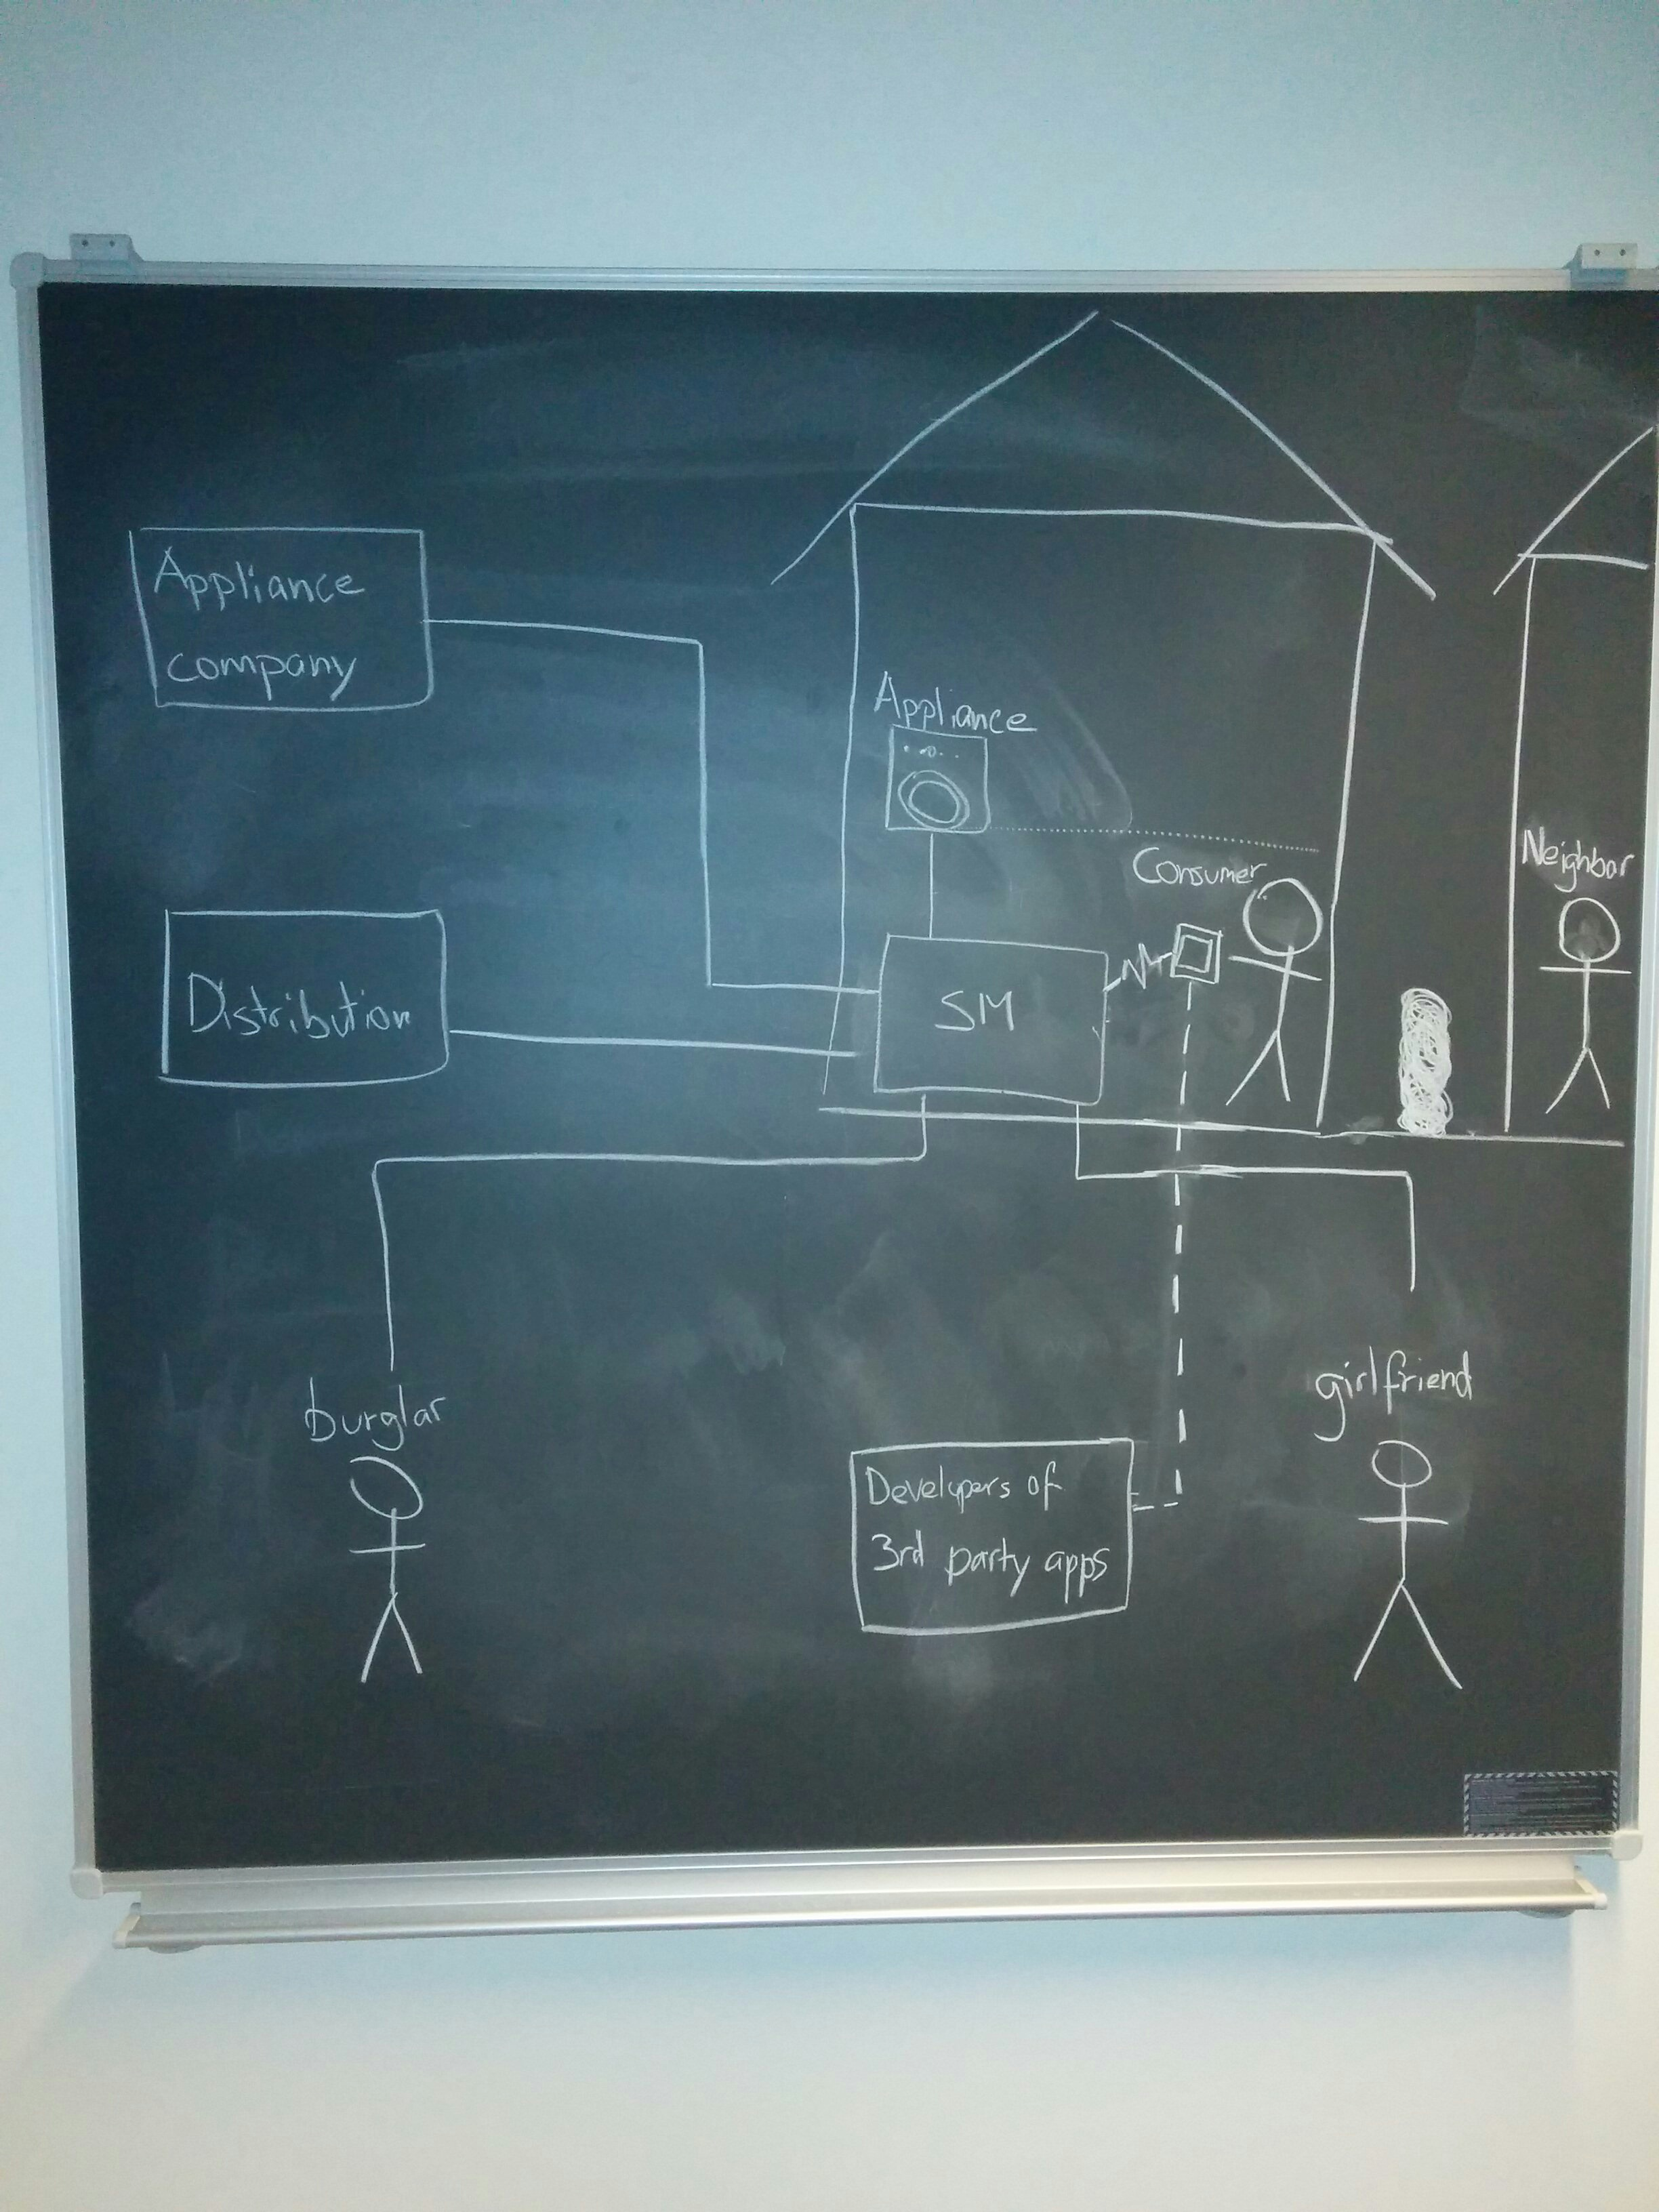
\includegraphics[width=0.5\textwidth]{figures/situation}
  \caption{Smart meter context model.}
  \label{contextual:sm_model}
\end{figure}

\paragraph{Actors}
Below is the listing of the actors represented in the full system and context.
As noted above, some of these actors are not represented visually in \cref{contextual:sm_model} but are part of the information flow of the entire system (see \cref{contextual:system}).
The listings below will not describe the potential threats in the system, but only list the possible actors involved in such threats.
\begin{itemize}
\item \textbf{Consumer}\\
The resident of the depicted home and the one which power consumption is monitored.
The smart meter is installed in the consumers home.

\item \textbf{Neighbor}\\
The next door neighbor to the consumer.
This person can also be viewed as a consumer and be expected to have a situation similar to the consumers.
However the neighbor is viewed only in the context of living near the consumer.
\item \textbf{Girlfriend}\\
The consumers girlfriend.
It is assumed that this is not a person that is living with the consumer.
\mikkel{Should we also have an actor that lives with the consumer? There might not be a treat in that but it is part of the model.}
\item \textbf{Burglar}\\ wants to find out when the consumer is home in order to break in, what products the consumer own in order to assess him as a target

\item \textbf{Power deliverance company}\\
The company billing the consumer for his power consumption.
\item \textbf{Power production company}\\
Produces the power and supplies it to the power grid.
This power production can be in the form of power plants or renewable energy.
\item \textbf{Power distribution company}\\
Manages the part of the grid closest to the consumer and provides him with electricity.
Installs the smart meters in the costumers home.
\item \textbf{Government}\\
The government officials (including counties and municipalities).

\item \textbf{Developers of third party apps}\\
the developer of apps that the consumer will use for seeing his electrical consumption. Can be both mobile, desktop and web applications
\item \textbf{Smart meter manufacturer}\\
\item \textbf{Appliance company}\\ the provider of home appliances that can collaborate with the SM.
\end{itemize}

\paragraph{Objects}\bruno{Better name!?}
\begin{itemize}
\item \textbf{Smart meter}\\ controls home appliances and also records consumption for each.
\item \textbf{Appliance}\\ has an option to be controlled from the smart meter. For instance a washing machine can be started and stopped when scheduled.
\end{itemize}

The smart meter is installed in the household of the consumer, in this case a house.
Home appliances are connected to the SM through their power cable, which provides electricty and information exchange.
The SM can be accessed through an API with different levels of rights, depending on the actor.
The consumer can access and manage his home appliances connected to the smart meter through some sort of program for instance an app, developed by a third party.
The girlfriend has access to the SM by having a password from the consumer or having her own account.
The distribution has the ability to update software, check the consumption and switch off the SM.
The home appliance company can update the firmware of their appliances through the SM.
The burglar and the Neighbour can try to access the SM through the API or physically at the household.

